\chapter{Introduction}

\section{Background}
\label{sec:background}

\subsection{Clear cell renal cell carcinoma(ccRCC)}
\label{subsec:Clear}

Renal cell carcinoma (RCC) makes up approximately 80\% of kidney cancer, and it is the seventh most common cancer in men and the ninth most common cancer in women\cite{rini_renal_2009}. RCC is thought to originate from cells in the proximal convoluted tubule of the nephron. A subtype named clear cell renal cell carcinoma (ccRCC) is the most common and aggressive form of RCC and we have little knowledge of the related tumor suppressor genes or oncogenes\cite{yang_gene_2017}. The surgical excision of the tumor or the whole kidney is a major approach to cure patients but it is not only limited by patients’condition but also kills the kidney function and has risk factors for recurrence after surgery. As a result, we need to investigate the underlying molecular mechanisms of ccRCC to develop potential targeted therapy.

Previous research shows that ccRCC is mostly characterized by the Von Hippel-Lindau (VHL) tumor suppressor gene mutation. VHL gene encodes the proteion pVHL, a recognition component of an E3-ubiquitin ligase complex. This complex targets hypoxia-inducible factor(HIF)-1α and HIF-2α for proteasomal degradation under normoxic conditions. The loss of the VHL gene function results in abnormal activation of HIF factors that participate in the glycolysis, angiogenesis and metastasis processes of tumor cells. However, the loss of VHL gene function alone is not sufficient to develop ccRCC\cite{sanchez_genetic_2018}. Another 3 chromatin modifying enzyme genes BAP1, PBRM1, and SETD2 are also frequently mutated in ccRCC based on the Cancer Genome Atlas (TCGA) data\cite{eckel-passow_8q24_2020}. There is also evidence that the PI3K / AKT / mTOR pathway contributes significantly to ccRCC prognosis. This pathway is typically regulated by other factors, such as miRNAs\cite{braga_molecular_2019}. Previous studies have also emphasized the important regulatory roles of long non-coding RNAs(lncRNAs)\cite{zeng_prognosis_2019} in ccRCC developments. However, ccRCC is a highly heterogeneous disease and the information available at this time is insufficient to provide a clear picture of the initiation and progression of the disease. The development of ccRCC can be linked to combinations of alterations at different levels, such as inactivation or abnormal expression levels of proteins, as well as alterations in regulatory elements, transcription factors involved in key pathways. Notably, nearly all those alterations are originally started by genetic mutations. Not only the ccRCC, but also other cancers are mostly driven by DNA-level variations. As a result, it is important to explore the cancers development that start at the DNA level.


\subsection{The aim of GWAS studies and eQTL analysis}

As the reason mentioned at the end of section \ref{subsec:Clear}, the research methods such as Genome-wide association studies (GWAS) have contributed to the discovery of disease-related genetic variations. The GWAS studies aim at scanning the genomes of populations to discover genetic markers that are used as predictors of a certain trait or disease. However, most of the identified single-nucleotide polymorphisms (SNPs) from GWAS studies fall within the non-coding region, which means they might only function as indirectly regulatory factors. The GWAS study uses a variety of diseases and traits as phenotypes, so GWAS ‘hit’ does not necessarily identify the gene, tissue, cell, or mechanism that mediates the direct biological effect\cite{sampson_glomerular_2019}. As a result, they cannot provide information about genes and pathways that directly relate to the risk loci.
 
The expression quantitative trait loci (eQTL) analysis is aiming at finding genetic variations (both SNPs or Indels) that directly control gene expression. It could be explained as a special genome-wide association study (GWAS) that uses quantitative gene expression levels as phenotypes. The figure \ref{Causal} is a nice illustration of relationship between GWAS and eQTL analysis. By performing eQTL analysis, it is possible to uncover genetic variants that regulate gene expression and construct gene regulatory networks. The eGenes, defined as genes that have at least one significant eQTL site, will provide a reference for driver disease genes identification. The eQTL analysis has been used in several relevant studies to explore the oncogenic mutation, risk loci, and pathway alterations in ccRCC. The eQTL study will connect mutations found in ccRCC patients with known gene regulation mechanisms, and also will open the possibility of uncovering novel mechanisms.

\begin{figure}[h]
\centering
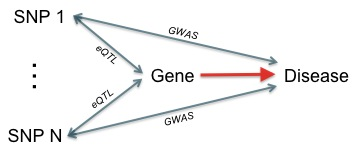
\includegraphics[width=0.5\textwidth]{figures/Causal.jpg}
\caption{A simple illustration for the relationship of SNPs,eQTLs,gene,GWAS and diseases(http://sherlock.ucsf.edu/).}
\label{Causal}
\end{figure}

\subsection{Existed healthy kidney eQTL analysis from GTEx using software FastQTL}

In recent years, eQTL-related databases and statistical methods have both been developed. The Genotype-Tissue Expression (GTEx) project includes eQTL analysis data on 54 non-disease tissues from 948 donors with over 15000 samples collected. In the GTEx version 8 release, there are 73 kidney-cortex samples with donor genotype information. The software packages which implement statistical methods of eQTL analysis for single tissue or single cell type are now relatively mature, such as Matrix eQTL\cite{shabalin_matrix_2012} and FastQTL\cite{ongen_fast_2016} improved based on Matrix eQTL. The latest GTEx cis eQTL mapping was performed using FastQTL.

In the GTEx portal((https://gtexportal.org/home/), the donor's kidney cortex tissues were collected and the eQTLs were analyzed using 73 samples. The donors usually died because of traumatic injury, cerebrovascular or heart disease, etc. Few of them have diseases related to the renal. This study provided a background of potential key genetic variations that regulate the kidney tissue's gene expression in the donor bodies but did not contribute to the landscape of specific diseases, such as ccRCC. This study majorly included White(84.6\%) subjects, followed by African American(12.9\%) ones, and only a small proportion of Asian(1.3\%) subjects were involved. As a result, there is also a lack of Asian targeted eQTLs in the GTEx database.

\subsection{Variants type appeared in cancer tissues}
\label{subsec:Variants type appeared in cancer tissues}

A lot of published cancer-related eQTL analyses have been published. Gene expression regulation in tumors is largely different from healthy tissue. Firstly, the tumor tissues usually carry lots of somatic mutations. The somatic mutations are not inherited by parents, but occur when cancer cells are developing. The somatic mutations could act either as "driver" mutations that are oncogenic or "passenger" mutations that promote the tumor lesions. The various types of mutations that appeared in cancer cells could be copy number variations, SNPs, Indels, and also epigenetic changes such as DNA methylation. The "driver" mutations bring growth advantage to the tumor cells and usually act as non-synonymous mutations in coding exons, and the "driver" genes are usually identified as protein kinase family\cite{greenman_patterns_2007}.

Besides, gene expression could also be affected by germline variants. Germline variants are usually applied to predict some inherited cancer's developing risks or assess drug sensitivity and toxicity for specific patients. Notably, the germline variants have been identified to have associations with cancer gene expression from a lot of studies such as a pan-cancer study in USA\cite{huang_pathogenic_2018} that identified the pathogenic germline mutations.

SNPs in different genome locations affect gene expression in different ways. SNPs within transcriptional regulatory elements might alter transcription efficiency, and SNPs within genes might change the mRNA splicing and mRNA stability to affect the detected transcripts and downstream translation(Robert and Pelletier, 2018). Some SNPs might regulate genes on larger distances and even different chromosomes. Most eQTL analyses focus on finding the cis-eQTLs that the SNPs act on local genes because the trans-eQTLs that act on distant genes tend to have weaker effects than cis-eQTLs and the detection requires a larger sample size and more calculations\cite{shan_identification_2019}.


\section{Methodology}

The variations in two different levels(germline level and somatic level) described in \ref{subsec:Variants type appeared in cancer tissues} brings the difficulties in cancer-related eQTLs analysis. In a research about breast cancer eQTLs\cite{li_integrative_2013}, the influence of somatic copy number variations and the DNA methylation was first considered in a multivariate linear model and the residual expression was regressed to the germline genotypes in order to find the germline risk loci. This model is able to assess the influence of 3 kinds of variations separately, however, it also needs additional data collection and processing for DNA methylation and copy number variations. A research about colon cancer eQTLs\cite{moreno_colon-specific_2018} has pointed out that the expression of genes in tumor tissues has changed greatly compared to normal, so the expression value from normal tissues was majorly used. The genotypes used in the colon study were from both adjacent normal colon tissues(obtained from cancer patients) and normal colon tissues(obtained from healthy volunteers). However, in this degree project, the gene expression of normal tissues was not available. In able to identify eQTLs in tumor tissues, several studies were focused on the somatic mutations inside the tumor samples. A research including multiple tumor types\cite{zhang_global_2018} was aimed at identifying somatic mutated "loci" in tumor samples that affect tumor gene expressions. They performed whole-genome sequencing for 930 tumors and grouped the mutations that close to each other within 50 bps into recurrently mutated loci. To achieve this union of adjacent mutations, huge sample size and deep sequencing depth were needed. 

The research about eQTLs in ccRCC diseases is relatively rare. A research\cite{yang_gene_2017} used the whole-exome sequencing data from 417 paired tumor and normal samples to get the somatic mutations. Then they used differential expressed gene modules to process the eQTL analysis, which generated from RNA-sequencing data from both tumor and normal tissues. 


\section{Goals}

This project’s main goal is to comprehensively understand the gene expression determinants in ccRCC and gain insights into the underlying biology of ccRCC development. In this study, existing sequencing data from the other research project are used, but are analyzed in a different manner. The eQTL analysis based on the provided ccRCC cancer cohort will able to give the information of SNPs that significantly affects the cancer tissue's gene expression. Furthermore, the eGenes that show high expression changes controlled by genotypes will reflect potential cancer-related cellular pathways. The unique population composition of this cohort will give more reference to Asia-specific ccRCC eQTLs. By comparing the identified kidney cancer eGenes with GTEx healthy kidney databases, special cancer-related eQTLs and eGenes are able to be discovered. This information will replenish current kidney tissue disease databases and provide potential strategies for drug development.